\chapter{Formal Analysis Using Alloy}

\section{Alloy Model}
In this section is presented a formal model of the CKB platform using alloy. The model is a simplification of the entire system and represent only the most significant parts.
\lstinputlisting[language=alloy]{CKBmodel.als}

\subsection*{World 1}
In world 1 (figure \ref{fig:world1}) are represented the interactions between multiple tournaments, multiple battles, and some educator and students.
\begin{sidewaysfigure}[h]
        \centering
        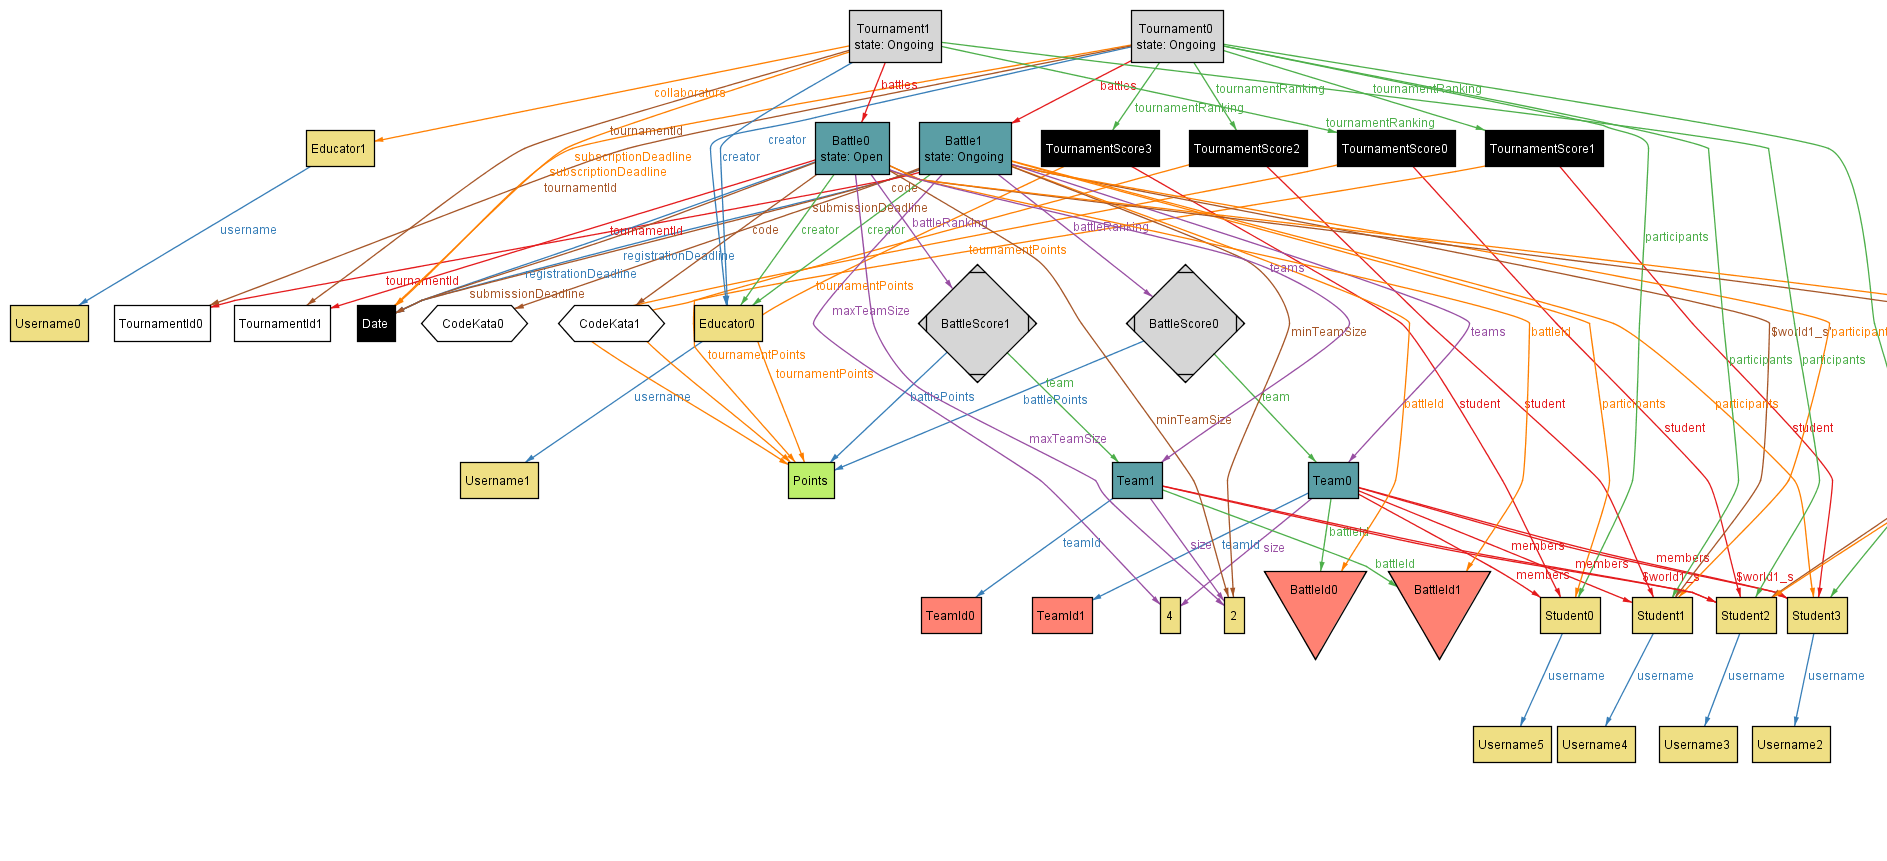
\includegraphics[scale=0.4]{images/W1.png}
        \caption{World 1}
        \label{fig:world1}
\end{sidewaysfigure}

\subsection*{World 2}
In world 2 (figure \ref{fig:world2}) is represented the score system (with rankings) and the team structure of a battle.
\begin{sidewaysfigure}[h]
        \centering
        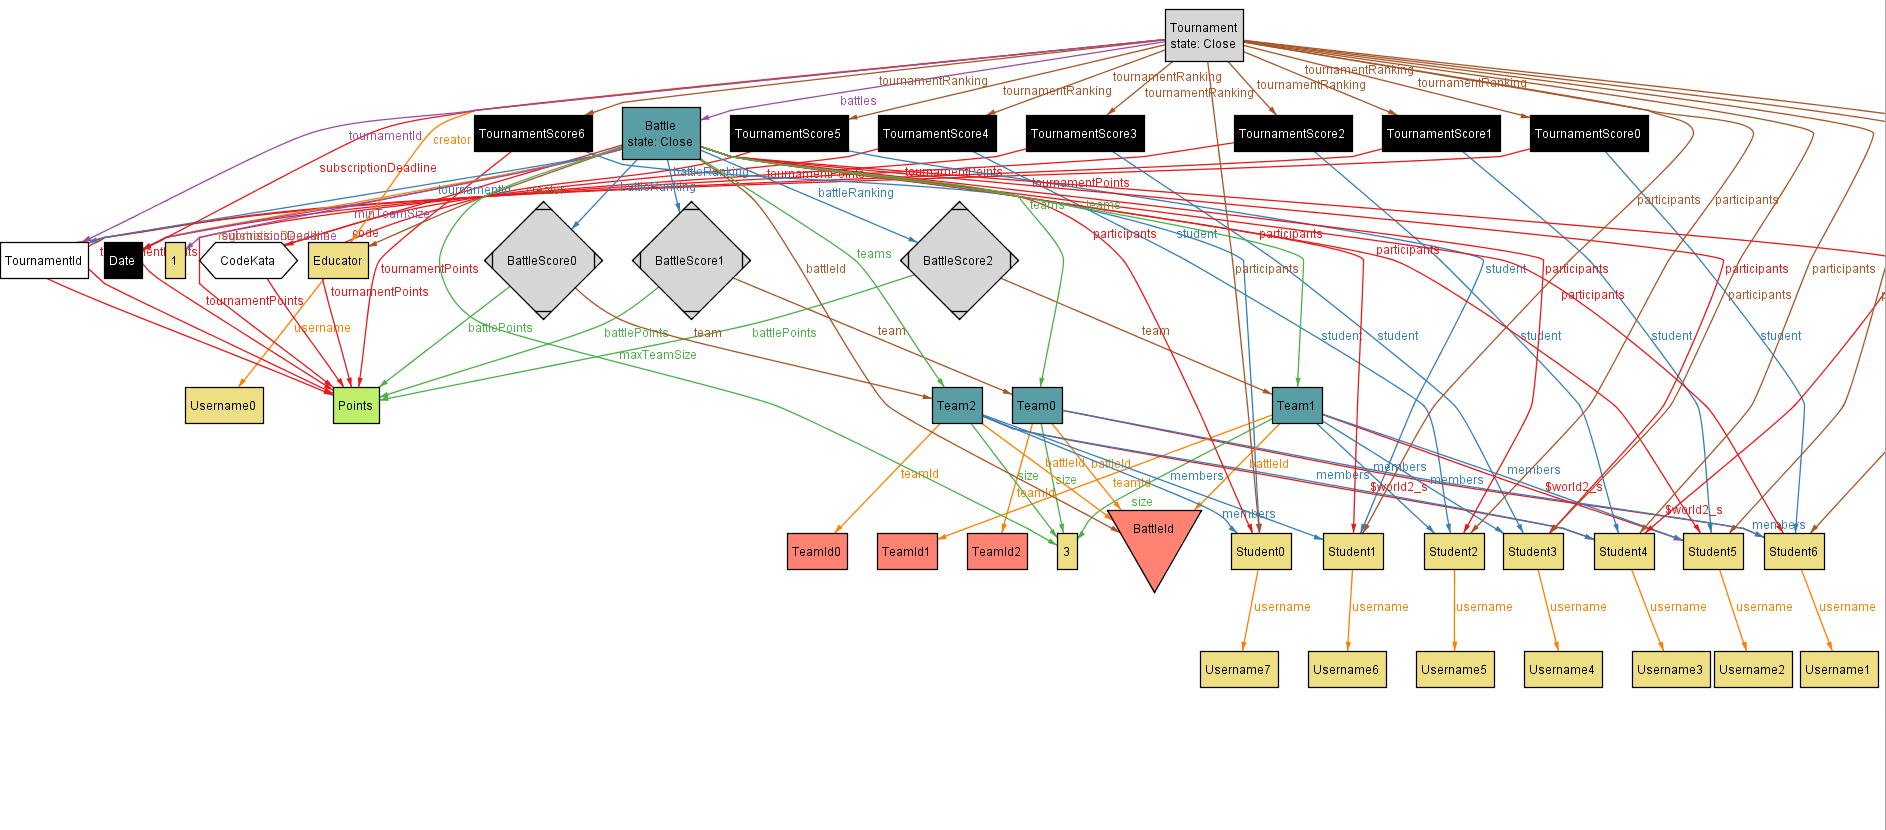
\includegraphics[scale = 0.4]{images/W2.png}
        \caption{World 2}
        \label{fig:world2}
\end{sidewaysfigure}

\subsection*{World 3}
In world 3 (figure \ref{fig:world3}) is represented the badge management and its assignment due to the tournament state.
\begin{sidewaysfigure}[h]
        \centering
        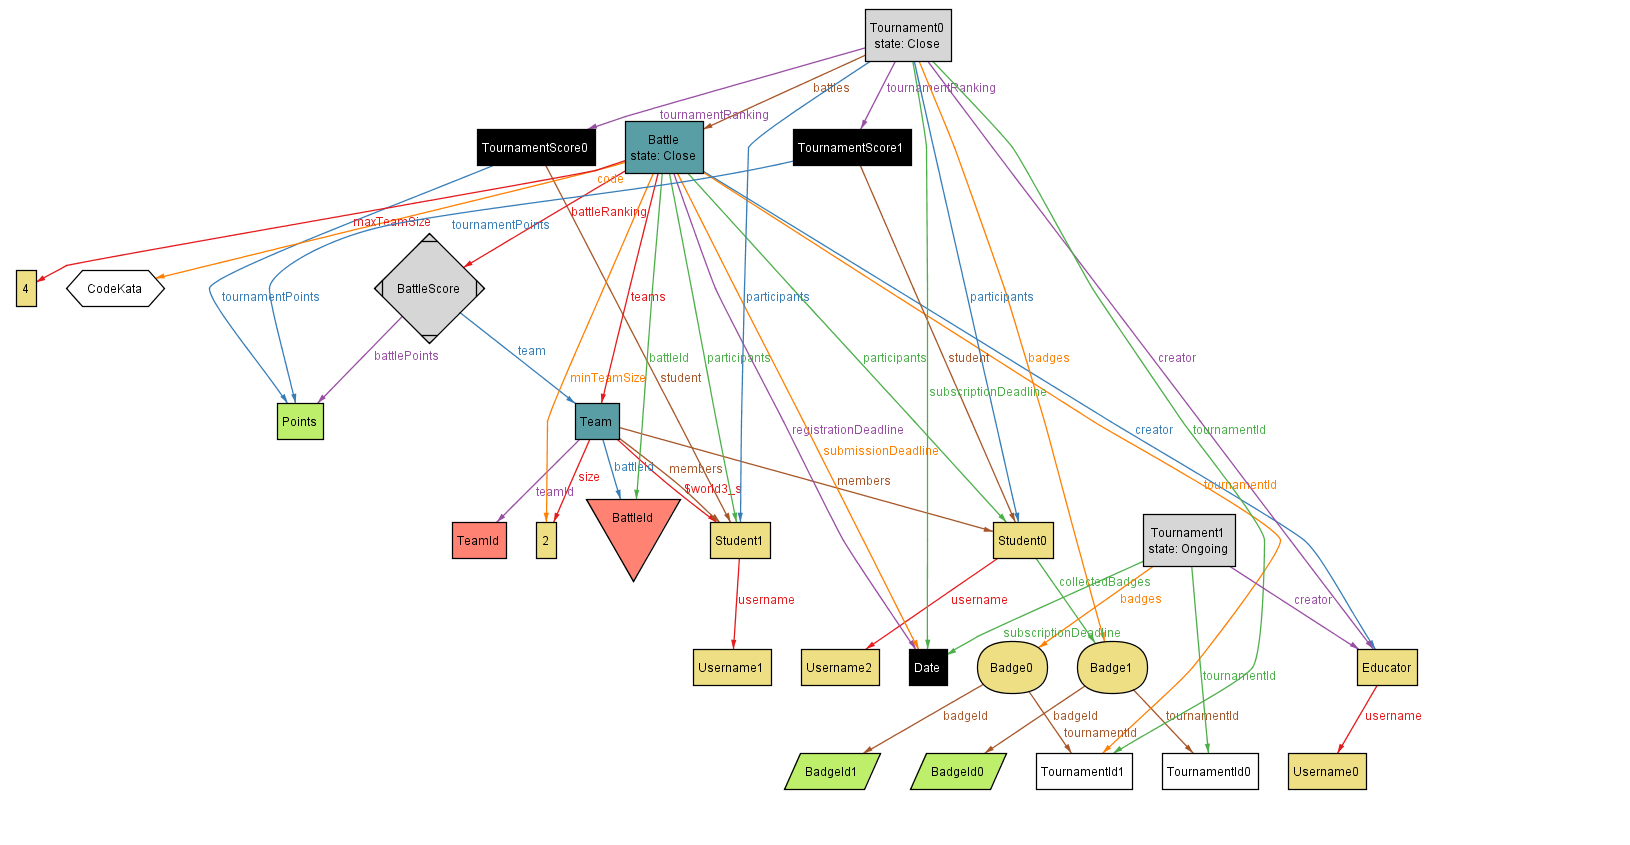
\includegraphics[scale = 0.5]{images/W3.png}
        \caption{World 3}
        \label{fig:world3}
\end{sidewaysfigure}
